% Parent preamble: \usepackage{graphicx,amsmath,booktabs} (and caption if floats are customized).
\setlength{\belowcaptionskip}{6pt}
\subsection{All-electron Kohn--Sham accuracy}

We next assess the accuracy of SPARC-atomSFE for all-electron Kohn--Sham DFT calculations through comparisons with literature codes. In particular, we consider four exchange-correlation functionals: LDA, PBE, rSCAN, and HF. For LDA, PBE, and rSCAN, results are compared for ten atoms ranging from light to heavy---H, Be, C, Ne, Na, Si, Fe, Kr, Gd, and U---against the FeAtom code for LDA and the atomPAW code for PBE and rSCAN. For HF, comparisons are carried out for closed-shell neutral atoms against Lehtola \textit{et al.}, and for charged species---anions $\mathrm{H}^{-}$, $\mathrm{Li}^{-}$, $\mathrm{F}^{-}$, $\mathrm{Na}^{-}$, $\mathrm{Cl}^{-}$ and cations $\mathrm{Li}^{+}$, $\mathrm{B}^{+}$, $\mathrm{Na}^{+}$, $\mathrm{Al}^{+}$---against Lehtola \textit{et al.} The distribution of the differences in the results is shown as violin plots in Figure~\ref{fig:ae-xc-accuracy-violin}. We observe that total energies and occupied eigenvalues agree to $10^{-6}$~Ha or better in most cases; the somewhat larger errors observed for PBE and rSCAN can likely be attributed to the accuracy of the atomPAW reference results (as we were unable to converge them further) rather than to SPARC-atomSFE itself, with rSCAN showing slightly worse agreement than PBE. Notably, for LDA, the total energy and eigenvalues of SPARC-atomSFE and FeAtom agree to $10^{-8}$~Ha and $10^{-9}$~Ha, respectively, even for the heaviest atom considered, U ($Z=92$). These results demonstrate the accuracy of SPARC-atomSFE for atomic structure calculations based on all-electron Kohn--Sham DFT.

\begin{figure}[!htbp]
    \centering
    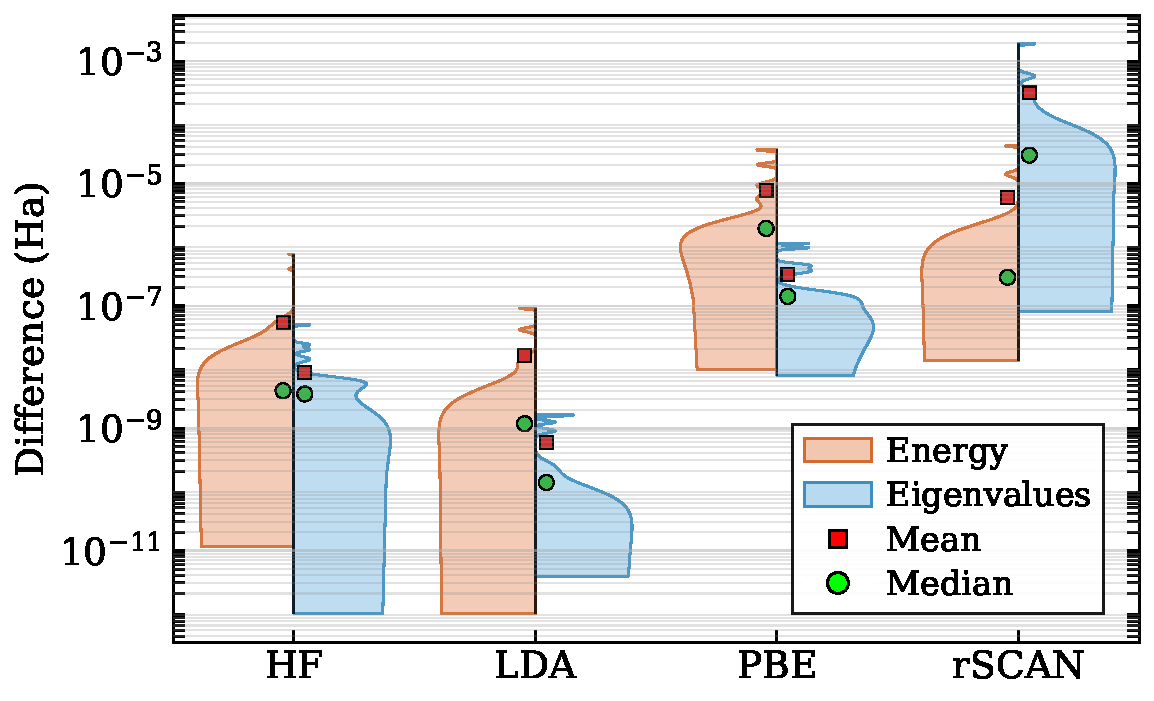
\includegraphics[width=\textwidth]{../figures/xc_accuracy_violin_ae}
    \caption{Comparison of SPARC-atomSFE all-electron Kohn--Sham DFT results with literature for various exchange-correlation functionals. The energy and eigenvalue errors denote the absolute differences in the corresponding quantities.}
    \label{fig:ae-xc-accuracy-violin}
\end{figure}

As supplementary material to the accuracy discussion above, we tabulate the full numerical data underlying Figure~\ref{fig:ae-xc-accuracy-violin}.

\begin{table}[!htbp]
    \centering
    \footnotesize
    \setlength{\tabcolsep}{3pt}
    \caption{Comparison of total energies and eigenvalues for the choice of LDA-SVWN exchange-correlation functional.}
    \label{tab:ae-acc-lda-svwn-rep10}
    \begin{tabular}{@{}c c ccc cc@{}}
        \toprule
        & & \multicolumn{3}{c}{$-E_{\mathrm{tot}}$ (Ha)} & \multicolumn{2}{c}{Occupied-eigenvalue Difference (Ha)} \\
        \cmidrule(lr){3-5} \cmidrule(lr){6-7}
        & $Z$ & atomSFE & FeAtom & Difference & Max $|\Delta \varepsilon|$ & Mean $|\Delta \varepsilon|$ \\
        \midrule
        H  &  1 & $0.44567051824$  & $0.44567051824$  & $9.29\times10^{-13}$ & $3.86\times10^{-12}$ & $3.86\times10^{-12}$ \\
        Be &  4 & $14.4472094741$  & $14.4472094740$  & $8.31\times10^{-11}$ & $3.10\times10^{-11}$ & $1.90\times10^{-11}$ \\
        C  &  6 & $37.4257485361$  & $37.4257485360$  & $1.98\times10^{-10}$ & $9.68\times10^{-11}$ & $4.20\times10^{-11}$ \\
        Ne & 10 & $128.233481270$  & $128.233481269$  & $7.44\times10^{-10}$ & $3.64\times10^{-10}$ & $2.17\times10^{-10}$ \\
        Na & 11 & $161.440060310$  & $161.440060309$  & $9.04\times10^{-10}$ & $6.99\times10^{-11}$ & $4.39\times10^{-11}$ \\
        Si & 14 & $288.198396604$  & $288.198396603$  & $1.48\times10^{-09}$ & $1.37\times10^{-11}$ & $8.03\times10^{-12}$ \\
        Fe & 26 & $1261.09305585$  & $1261.09305584$  & $5.67\times10^{-09}$ & $2.04\times10^{-09}$ & $1.26\times10^{-09}$ \\
        Kr & 36 & $2750.14794043$  & $2750.14794042$  & $1.22\times10^{-08}$ & $1.50\times10^{-09}$ & $9.08\times10^{-10}$ \\
        Gd & 64 & $10816.6538772$  & $10816.6538772$  & $4.09\times10^{-08}$ & $2.37\times10^{-09}$ & $1.67\times10^{-09}$ \\
        U  & 92 & $25658.4178889$  & $25658.4178888$  & $9.18\times10^{-08}$ & $2.67\times10^{-09}$ & $1.63\times10^{-09}$ \\
        \bottomrule
    \end{tabular}
\end{table}

\begin{table}[!htbp]
    \centering
    \footnotesize
    \setlength{\tabcolsep}{3pt}
    \caption{Comparison of total energies and eigenvalues for the choice of PBE exchange-correlation functional.}
    \label{tab:ae-acc-pbe-rep10}
    \begin{tabular}{@{}c c ccc cc@{}}
        \toprule
        & & \multicolumn{3}{c}{$-E_{\mathrm{tot}}$ (Ha)} & \multicolumn{2}{c}{Occupied-eigenvalue Difference (Ha)} \\
        \cmidrule(lr){3-5} \cmidrule(lr){6-7}
        & $Z$ & atomSFE & atomPAW & Difference & Max $|\Delta \varepsilon|$ & Mean $|\Delta \varepsilon|$ \\
        \midrule
        H  &  1 & $0.458928588$   & $0.458928597$   & $9.13\times10^{-09}$ & $7.22\times10^{-09}$ & $7.22\times10^{-09}$ \\
        Be &  4 & $14.62994793$   & $14.62994772$   & $2.14\times10^{-07}$ & $9.80\times10^{-08}$ & $5.27\times10^{-08}$ \\
        C  &  6 & $37.74820924$   & $37.74820878$   & $4.55\times10^{-07}$ & $4.04\times10^{-08}$ & $2.95\times10^{-08}$ \\
        Ne & 10 & $128.8664291$   & $128.8664277$   & $1.38\times10^{-06}$ & $1.34\times10^{-07}$ & $9.12\times10^{-08}$ \\
        Na & 11 & $162.1645960$   & $162.1645945$   & $1.55\times10^{-06}$ & $2.51\times10^{-07}$ & $1.32\times10^{-07}$ \\
        Si & 14 & $289.2027550$   & $289.2027529$   & $2.13\times10^{-06}$ & $5.84\times10^{-07}$ & $1.53\times10^{-07}$ \\
        Fe & 26 & $1263.295438$   & $1263.295432$   & $5.63\times10^{-06}$ & $2.21\times10^{-06}$ & $3.70\times10^{-07}$ \\
        Kr & 36 & $2753.416118$   & $2753.416109$   & $9.33\times10^{-06}$ & $1.37\times10^{-06}$ & $4.58\times10^{-07}$ \\
        Gd & 64 & $10823.19862$   & $10823.19860$   & $2.03\times10^{-05}$ & $8.75\times10^{-06}$ & $1.06\times10^{-06}$ \\
        U  & 92 & $25668.41171$   & $25668.41167$   & $3.53\times10^{-05}$ & $1.05\times10^{-05}$ & $8.92\times10^{-07}$ \\
        \bottomrule
    \end{tabular}
\end{table}

\begin{table}[!htbp]
    \centering
    \footnotesize
    \setlength{\tabcolsep}{3pt}
    \caption{Comparison of total energies and eigenvalues for the choice of rSCAN exchange-correlation functional.}
    \label{tab:ae-acc-rscan-rep10}
    \begin{tabular}{@{}c c ccc cc@{}}
        \toprule
        & & \multicolumn{3}{c}{$-E_{\mathrm{tot}}$ (Ha)} & \multicolumn{2}{c}{Occupied-eigenvalue Difference (Ha)} \\
        \cmidrule(lr){3-5} \cmidrule(lr){6-7}
        & $Z$ & atomSFE & atomPAW & Difference & Max $|\Delta \varepsilon|$ & Mean $|\Delta \varepsilon|$ \\
        \midrule
        H  &  1 & $0.452860365$   & $0.452860352$   & $1.27\times10^{-08}$ & $7.97\times10^{-08}$ & $7.97\times10^{-08}$ \\
        Be &  4 & $14.65119802$   & $14.65119794$   & $8.55\times10^{-08}$ & $8.66\times10^{-06}$ & $4.68\times10^{-06}$ \\
        C  &  6 & $37.76635704$   & $37.76635699$   & $5.21\times10^{-08}$ & $1.34\times10^{-05}$ & $5.75\times10^{-06}$ \\
        Ne & 10 & $128.9723925$   & $128.9723925$   & $4.62\times10^{-08}$ & $5.24\times10^{-05}$ & $2.29\times10^{-05}$ \\
        Na & 11 & $162.2862159$   & $162.2862160$   & $6.15\times10^{-08}$ & $6.51\times10^{-05}$ & $2.19\times10^{-05}$ \\
        Si & 14 & $289.3767993$   & $289.3767988$   & $5.01\times10^{-07}$ & $1.22\times10^{-04}$ & $3.51\times10^{-05}$ \\
        Fe & 26 & $1263.668535$   & $1263.668536$   & $1.04\times10^{-06}$ & $6.72\times10^{-04}$ & $1.53\times10^{-04}$ \\
        Kr & 36 & $2754.194549$   & $2754.194547$   & $1.16\times10^{-06}$ & $1.39\times10^{-03}$ & $2.97\times10^{-04}$ \\
        Gd & 64 & $10824.64115$   & $10824.64117$   & $1.42\times10^{-05}$ & $3.08\times10^{-03}$ & $5.69\times10^{-04}$ \\
        U  & 92 & $25670.94593$   & $25670.94589$   & $4.13\times10^{-05}$ & $1.42\times10^{-02}$ & $1.92\times10^{-03}$ \\
        \bottomrule
    \end{tabular}
\end{table}

\begin{table}[!htbp]
    \centering
    \footnotesize
    \setlength{\tabcolsep}{3pt}
    \caption{Hartree--Fock closed-subshell benchmark for 17 atoms: SPARC-atomSFE vs.\ Lehtola \textit{et al.}
    Entries are total energy $E_{\mathrm{tot}}$, HOMO eigenvalue $\varepsilon_{\mathrm{HOMO}}$, and exchange energy $E_x$ (Ha).}
    \label{tab:ae-hf-closed-subshell}
    \resizebox{\linewidth}{!}{%
    \begin{tabular}{@{}c c ccc ccc ccc@{}}
        \toprule
        & & \multicolumn{3}{c}{$-E_{\mathrm{tot}}$ (Ha)} & \multicolumn{3}{c}{$-\varepsilon_{\mathrm{HOMO}}$ (Ha)} & \multicolumn{3}{c}{$-E_{\mathrm{x}}$ (Ha)} \\
        \cmidrule(lr){3-5} \cmidrule(lr){6-8} \cmidrule(lr){9-11}
        & $Z$ & atomSFE & Lehtola & Difference & atomSFE & Lehtola & Difference & atomSFE & Lehtola & Difference \\
        \midrule
        He &  2 & $2.861679995600$ & $2.861679995612$ & $1.17\times10^{-11}$ & $0.91795556285$ & $0.91795556286$ & $2.57\times10^{-12}$ & $1.025768869910$ & $1.025768869900$ & $1.04\times10^{-11}$ \\
        Be &  4 & $14.57302316828$ & $14.57302316832$ & $3.60\times10^{-11}$ & $0.30926955153$ & $0.30926955157$ & $4.15\times10^{-11}$ & $2.666913669350$ & $2.666913669390$ & $3.96\times10^{-11}$ \\
        Ne & 10 & $128.5470981088$ & $128.5470981094$ & $5.79\times10^{-10}$ & $0.85040965035$ & $0.85040965035$ & $9.37\times10^{-13}$ & $12.10835073105$ & $12.10835073117$ & $1.15\times10^{-10}$ \\
        Mg & 12 & $199.6146364237$ & $199.6146364245$ & $7.70\times10^{-10}$ & $0.25305258176$ & $0.25305258201$ & $2.51\times10^{-10}$ & $15.99429168655$ & $15.99429168694$ & $3.91\times10^{-10}$ \\
        Ar & 18 & $526.8175128010$ & $526.8175128027$ & $1.76\times10^{-9}$ & $0.59101740571$ & $0.59101740935$ & $3.64\times10^{-9}$ & $30.18494199109$ & $30.18494198731$ & $3.78\times10^{-9}$ \\
        Ca & 20 & $676.7581859224$ & $676.7581859245$ & $2.12\times10^{-9}$ & $0.19552969154$ & $0.19552969247$ & $9.30\times10^{-10}$ & $35.21120850330$ & $35.21120850517$ & $1.87\times10^{-9}$ \\
        Zn & 30 & $1777.848116185$ & $1777.848116191$ & $6.10\times10^{-9}$ & $0.29250714776$ & $0.29250714640$ & $1.36\times10^{-9}$ & $69.64119795154$ & $69.64119795404$ & $2.50\times10^{-9}$ \\
        Kr & 36 & $2752.054977337$ & $2752.054977346$ & $8.62\times10^{-9}$ & $0.52418666755$ & $0.52418668103$ & $1.35\times10^{-8}$ & $93.85599601220$ & $93.85599600354$ & $8.66\times10^{-9}$ \\
        Sr & 38 & $3131.545686429$ & $3131.545686439$ & $9.30\times10^{-9}$ & $0.17845644076$ & $0.17845644685$ & $6.09\times10^{-9}$ & $101.9500832606$ & $101.9500832705$ & $9.84\times10^{-9}$ \\
        Pd & 46 & $4937.921024056$ & $4937.921024070$ & $1.44\times10^{-8}$ & $0.33600200815$ & $0.33600201367$ & $5.52\times10^{-9}$ & $139.1429137365$ & $139.1429137267$ & $9.78\times10^{-9}$ \\
        Cd & 48 & $5465.133142514$ & $5465.133142530$ & $1.57\times10^{-8}$ & $0.26485590698$ & $0.26485591255$ & $5.58\times10^{-9}$ & $148.9142513282$ & $148.9142513291$ & $9.70\times10^{-10}$ \\
        Xe & 54 & $7232.138363852$ & $7232.138363872$ & $1.95\times10^{-8}$ & $0.45729006132$ & $0.45729005785$ & $3.47\times10^{-9}$ & $179.0971093189$ & $179.0971093669$ & $4.80\times10^{-8}$ \\
        Ba & 56 & $7883.543827310$ & $7883.543827330$ & $2.09\times10^{-8}$ & $0.15752769303$ & $0.15752769864$ & $5.61\times10^{-9}$ & $189.1002498282$ & $189.1002498415$ & $1.33\times10^{-8}$ \\
        Yb & 70 & $13391.45619308$ & $13391.45619312$ & $3.60\times10^{-8}$ & $0.18246254162$ & $0.18246252223$ & $1.94\times10^{-8}$ & $276.2138392544$ & $276.2138392265$ & $2.79\times10^{-8}$ \\
        Hg & 80 & $18408.99149490$ & $18408.99149494$ & $4.50\times10^{-8}$ & $0.26104596502$ & $0.26104601419$ & $4.92\times10^{-8}$ & $345.3035177000$ & $345.3035163829$ & $1.32\times10^{-6}$ \\
        Rn & 86 & $21866.77224082$ & $21866.77224087$ & $5.30\times10^{-8}$ & $0.42800677179$ & $0.42800676968$ & $2.12\times10^{-9}$ & $387.5037738100$ & $387.5037737909$ & $1.91\times10^{-8}$ \\
        Ra & 88 & $23094.30366637$ & $23094.30366642$ & $5.50\times10^{-8}$ & $0.14877117348$ & $0.14877119673$ & $2.33\times10^{-8}$ & $401.4148473300$ & $401.4148474301$ & $1.00\times10^{-7}$ \\
        \bottomrule
    \end{tabular}%
    }
\end{table}

\begin{table}[htbp]
    \centering
    \footnotesize
    \setlength{\tabcolsep}{4pt}
    \caption{Hartree--Fock charged benchmark: SPARC-atomSFE vs.\ Lehtola \textit{et al.}
    Values are reported as $-E_{\mathrm{tot}}$ (Ha). Since the reference table is reported to 9 digits after the decimal point, the absolute total-energy errors are computed from these rounded values and reported with conservative precision.}
    \label{tab:ae-hf-charged-unpolarized}
    \begin{tabular}{@{}c c c r@{.}l r@{.}l r@{}}
        \toprule
         & $Z$ & $N_e$ & \multicolumn{2}{c}{atomSFE} & \multicolumn{2}{c}{Lehtola} & \multicolumn{1}{c}{Difference} \\
        \midrule
        H$^{-}$  &  1 &  2 & 0   & 487929734 & 0   & 487929734 & $<1\times10^{-9}$ \\
        Li$^{+}$ &  3 &  2 & 7   & 236415201 & 7   & 236415201 & $<1\times10^{-9}$ \\
        Li$^{-}$ &  3 &  4 & 7   & 428231641 & 7   & 428232061 & $\phantom{<}4\times10^{-7}$ \\
        B$^{+}$  &  5 &  4 & 24  & 237575184 & 24  & 237575184 & $<1\times10^{-9}$ \\
        F$^{-}$  &  9 & 10 & 99  & 459453912 & 99  & 459453913 & $\phantom{<}1\times10^{-9}$ \\
        Na$^{+}$ & 11 & 10 & 161 & 676962614 & 161 & 676962614 & $<1\times10^{-9}$ \\
        Na$^{-}$ & 11 & 12 & 161 & 855125277 & 161 & 855125996 & $\phantom{<}7\times10^{-7}$ \\
        Al$^{+}$ & 13 & 12 & 241 & 674670464 & 241 & 674670465 & $\phantom{<}1\times10^{-9}$ \\
        Cl$^{-}$ & 17 & 18 & 459 & 576925266 & 459 & 576925268 & $\phantom{<}2\times10^{-9}$ \\
        \bottomrule
    \end{tabular}
\end{table}
